\documentclass[pdf,mpa]{prosper}

\FontText{\usefont{T1}{phv}{m}{n}\fontsize{16.4pt}{16pt}%
  \selectfont}{%
  \usefont{T1}{phv}{m}{n}\fontsize{16.4pt}{16pt}\selectfont}

\NewSlideStyle[13.5cm]{t}{5.5,3.5}{}



\usepackage{german}
\usepackage{amsfonts,amsmath}
\usepackage{url}
\usepackage[dvips]{graphicx}
\usepackage[latin1]{inputenc}

\usepackage[all,cmtip,ps,line,dvips]{xy}


\raggedright

% \newcommand{\kopf}[1]{{\tiny\tt #1} \par}
\newcommand{\kopf}[1]{}
\newcommand{\titel}[1]{\underline{\Large {#1}}}

\newcommand{\CF}{\mathsf{CF}}
\newcommand{\REG}{\mathsf{REG}}
\newcommand{\SL}{\mathsf{SL}}
\newcommand{\ZZ}{\mathbb{Z}}
\newcommand{\NN}{\mathbb{N}}

\newcommand{\FC}{\mathsf{FC}}
\newcommand{\RC}{\mathsf{RC}}
\newcommand{\RRC}{\mathsf{RRC}}
\newcommand{\OVL}{\mathsf{OVL}}
\newcommand{\Nf}{\mathsf{Nf}}


\title{
  The Leipzig \emph{autotool} E-Learning/E-Testing system
}
\author{ 
  Mirko Rahn, Univ. Karlsruhe \\
  Alf Richter, Univ. Leipzig \\
  \emph{Johannes Waldmann}, HTWK Leipzig
}  
\slideCaption{Math Tutoring Symposium, Heerlen 08}


\begin{document}
\maketitle

\begin{slide}{Beispiel: Graphenf�rbung (Aufgabe)}

\begin{minipage}{0.4\textwidth}
\includegraphics[width=7cm]{536970904.Dot.eps}
\end{minipage}%
\begin{minipage}{0.5\textwidth}
\begin{small}
\begin{verbatim}
Gesucht ist eine konfliktfreie 
Knoten-F�rbung des Graphen
Graph { knoten = mkSet [ 1 , 2 , 3 , 4 , 5 , 6 , 7 , 8 , 9 , 10 ]
  , kanten = mkSet [ kante 1 6 , kante 1 7 , kante 1 9 , kante 2 5
     , kante 2 7 , kante 2 8 , kante 2 9 , kante 3 6 , kante 3 7
     , kante 3 8 , kante 3 9 , kante 4 5 , kante 4 6 , kante 4 7
     , kante 5 6 , kante 5 10 , kante 6 7 , kante 6 8 , kante 6 10
     , kante 8 9 , kante 8 10 , kante 9 10 
     ] 
  }
mit h�chstens 3 verschiedenen Farben.
\end{verbatim}
\end{small}  
\end{minipage}

\end{slide}

\begin{slide}{Beispiel: Graphenf�rbung (L�sung)}
Eingabe:
\begin{small}
\begin{verbatim}
listToFM [ ( 1 , C ) , ( 2 , C ) , ( 3 , B ) , ( 4 , B ) , ( 5 , B )
    , ( 6 , A ) , ( 7 , A ) , ( 8 , C ) , ( 9 , C ) , ( 10 , C ) 
\end{verbatim}
\end{small}
Bewertung:
\begin{small}
\begin{verbatim}
Ist die Menge
    Knotenmenge des Graphen =
    mkSet [ 1 , 2 , 3 , 4 , 5 , 6 , 7 , 8 , 9 , 10 ]
Teilmenge der Menge
    gef�rbte Knoten = mkSet [ 1 , 2 , 3 , 4 , 5 , 6 , 7 , 8 , 9 , 10 ]
? Ja.
Diese Kante(n) verlaufen zwischen gleichfarbigen Knoten:
    [ kante 1 9 , kante 2 8 , kante 2 9 , kante 4 5 , kante 6 7
    , kante 8 9 , kante 8 10 , kante 9 10 ]
\end{verbatim}
\end{small}

\end{slide}

\begin{slide}{Typische Anwendung}

Problem (Bsp: 3SAT)
\begin{itemize}
\item Instanz: eine Formel in 3-KNF
\item L�sung: eine erf�llende Belegung
\end{itemize}

Ablauf mit \autotool\ :
\begin{itemize}
\item Tutor konfiguriert Generator
\item \autotool\ w�rfelt Instanz
  (f�r jeden Studenten eine andere)
\item Student gibt (vermutete) L�sung ein
\item \autotool\ verifiziert L�sung,
  gibt ausf�hrlichen Bericht (sofort)
\end{itemize}

\end{slide}




\begin{slide}{Beispiel: Graphenf�rbung (Konfiguration)}

das hat der Tutor eingestellt:
\begin{itemize}
\item Semantik:
Aufgabentyp: \verb|Col-Quiz| und Parameter
\begin{verbatim}
Config { nodes = 10 , edges = 30 , chi = 3 }
\end{verbatim}
\item Verwaltung:

Hochschule, Vorlesung, Aufgabe, Bearbeitungszeitraum, Wichtigkeit
\end{itemize}



\end{slide}

\begin{slide}{Problem levels}

problems are marked as
\begin{itemize}
\item Demo (``too easy'', for illustration)
\item Mandatory (must submit at least one correct solution before deadline,
  any number of attempts)
\item Optional (``too hard'', prize questions etc.)
\end{itemize}

even after deadline, student can
\begin{itemize}
\item
  work on problems (will be graded, but not counted)
\item
  review previous graded answer
\end{itemize}
useful e.g. when preparing for exams

\end{slide}


\begin{slide}{Aufgaben-Themen}

\begin{itemize}
\item
  formale Sprachen:

  Grammatiken (alle Chomsky-Typen), regul�re Ausdr�cke
\item
  Automaten/Berechnungsmodelle:

  endlich (Wort, Baum), Keller, Turing, Registermaschine,

  (primitiv) rekursive Funktionen
\item
  Graphen:   Parameter, F�rbungen, Wege, \dots
\item
  diskrete Mathematik und Logik: Zahlensysteme, \dots
\item
  Datenstrukturen: Suchb�ume, \dots
\end{itemize}

\end{slide}

\begin{slide}{\autotool\ as a verifier}

\begin{itemize}
\item
  ideally, problem is in NP (e.g. COL):
  \begin{itemize}
  \item
    student has to guess (N)
  \item
    \autotool\ has to check (P)
  \end{itemize}
\item
  sometimes solutiones are a bit longer (PCP)
\item
  or verification takes a bit longer 
  (equivalence of regular expressions)
\item
  sometimes verification is impossible,

  then replaced by testing (equivalence of CFG)
\end{itemize}

lots of opportunities to discuss with students
about decidability and complexity
\end{slide}


% \begin{slide}{Wichtige Datentypen}

(f�r Automaten und Sprachen)
\begin{itemize}
\item endlicher Automat, Kellerautomat
\item Grammatik
\item regul�rer Ausdruck
\end{itemize}

Repr�sentation m�glichst nahe an der mathematischen Wahrheit,

statt Tupel benutze Strukturen mit benannten Komponenten,

geschweifte Klammern sind daf�r reserviert,
deswegen Mengen als \verb|mkSet [ 1, 2, 3 ]|

\end{slide}


% \begin{slide}{Endliche Automaten}

\begin{small}
\begin{verbatim}
NFA { alphabet = mkSet "ab" , states = mkSet [ 1, 2, 3 ]
    , starts = mkSet [ 2 ] , finals = mkSet [ 2 ]
    , trans = collect 
          [ ( 1, 'a', 2 ), ( 2, 'a', 1 )
          , ( 2, 'a', 3 ), ( 2, 'b', 3 ), ( 3, 'b', 2 )
          ]
    }
\end{verbatim}
\end{small}  

Eigenschaften 
(f�r Test der Einsendungen und ggf. Konfiguration der Generatoren)

\begin{verbatim}
   Min_Size Int | Max_Size Int 
 | Alphabet ( Set c )
 | Deterministic | Minimal | Complete | Reduced 
\end{verbatim}
  
\end{slide}

% \begin{slide}{Regul�re Ausdr�cke}

\begin{verbatim}
((ba)^* + (bb)^*)^* + (ab)^*
\end{verbatim}

Definition:
\begin{itemize}
\item
  atomar: Buchstabe oder Name (\verb|Sigma, All|)
\item 
  zusammengesetzt mit Operationen:

  Verkettung (\verb|.|), Vereinigung \verb|+|, 
  Durchschnitt \verb|&|, Differenz \verb|-|,
  symmetrische Differenz \verb|<>|,
  Shuffle \verb|$|, Quotienten \verb|\,/|,
  Potenzen \verb|^int, ^*, ^+|
\end{itemize}

Eigenschaften:
\begin{verbatim}
   Min_Size Int | Max_Size Int | Alphabet ( Set c )
  | Simple -- nur Plus, Mal, Stern
  | Extended -- alles
\end{verbatim}


\end{slide}

% \begin{slide}{Grammatiken}

\begin{small}
\begin{verbatim}
Grammatik { terminale = mkSet "01"
          , variablen = mkSet "ST"
	  , start = 'S'
	  , regeln = mkSet [ ( "S", "" ), ( "S", "T0S" ), ( "T", "11" ) ]
	  }
\end{verbatim}
\end{small}  

Eigenschaften:
\begin{itemize}
\item monoton, kontextsensitiv, kontextfrei, linear, rechts/links-linear, 
\item f�r CFG: epsilon-frei, ketten-frei, Chomsky-normal, Greibach-normal
\item eindeutig (nat�rlich nur Test)
\end{itemize}


\end{slide}

\begin{slide}{Eine clevere L�sung}

\newcommand{\reverse}{\mathop{\textrm{reverse}}}

Aufgabe war: finde (kleine) CFG f�r
$L = \Sigma^* \setminus \{w w \mid  w \in\Sigma^* \}$
f�r $\Sigma=\{0,1\}$.

Die wesentliche Idee der L�sung ist:
\begin{itemize}
\item $L \to AB, L \to BA$ (start)
\item $A \to 0, A \to SAS$ (in der Mitte eine 0)
\item $B \to 1, B \to SBS$ (in der Mitte eine 1)
\item $S \to 0,S \to 1$ (ein beliebiges Zeichen)
\end{itemize}
jetzt fehlt aber noch etwas triviales.

Wie schafft man das mit nur zwei (nicht drei) weiteren Regeln?

\end{slide}

\begin{slide}{Fun with Regular Expressions (I)}

of course this works:
\begin{itemize}
\item given an extended reg. exp.
  (complement, intersection, shuffle, \dots)
\item find an equivalent simple reg. exp.
\end{itemize}
but finding a \emph{small} answer is hard (PSPACE?)

\newcommand{\shuffle}{\mathbin{\raisebox{8pt}{\rotatebox{-90}{$\exists$}}}}

try $a^{2*} \shuffle b^{2*}$ and then $a^{2*} \shuffle b^{2*} \shuffle c^{2*}$ 

\end{slide}

\begin{slide}{Fun with Regular Expressions (II)}

star height of an expression: maximal nesting number of stars

(extended) star height of a language: 
minimal star height of equiv. (extended) reg. exp.

\newcommand{\REG}{\operatorname{REG}}
\newcommand{\ESH}{\operatorname{ESH}}
Conjecture: $L\in\REG \Rightarrow \ESH(L)\le 1$.

exercise:
\begin{itemize}
\item given any (simple) reg. exp.
\item find equiv. extended reg. exp. of ESH $\le 1$
\end{itemize}

\end{slide}


\begin{slide}{Einsatz in Lehrveranstaltungen}

\begin{itemize}
\item
  Automaten und Sprachen (Uni Leipzig, 2001--2004)
\item
  Berechenbarkeit und Komplexit�t (Uni L)
\item
  Automaten und Sprachen im Compilerbau (HTWK Leipzig, 2003--)
\item
  Automaten und Sprachen in Grundlagen der Informatik (Nebenfach)
  (HTWK L)
\item
  Datenstrukturen, diskrete Mathematik in Grundlagen der Informatik (Nebenfach)
  (HTWK L)
\item
  Datenstrukturen, disk. Math. in Grundl. Inf. (Nebenfach)
  (Uni Karlsruhe, 2005)
\end{itemize}

(an HTWK) f�r ca. 150 Studenten gleichzeitig

\end{slide}

\begin{slide}{Erfahrungen}

\begin{itemize}
\item
  \autotool\ zur Unterst�tzung des �bungsbetriebes.

  etwa die H�lfte der Aufgaben mit \autotool\ korrigieren
  \dots die andere H�lfte: schriftliche (Beweis-)Aufgaben
\item
  wird von Studenten gut angenommen, 

  sind erfreut �ber sofortige, ausf�hrliche Antwort.
\item
  Highscore-Wertung (mit Preisen) schafft zus�tzlichen Anreiz
\item
\end{itemize}

\end{slide}


\begin{slide}{Requirements}

Client (student, tutor): any web browser

Server:
\begin{itemize}
\item 
  for running: standard GNU/Linux machine with (Apache) web server,
  MySQL data base server 
\item for building: GHC Haskell compiler, some libraries (from hackage)
\item
  tricky parts (currently not well-documented):
  build from source, initialize data base
\item one central server can be used for several institutions
  with several lectures each
\end{itemize}


\end{slide}

\begin{slide}
\titel{Bestandteile}

\begin{itemize}
\item
  Semantik-Module (Automaten, Grammatiken, Graphen, \dots)
\item
  Generatoren f�r Aufgaben
\item
  Korrektoren f�r Einsendungen
\item
  Datenbank f�r Konfiguration der Aufgaben bzw. Generatoren, 
  erreichte Punkte
\item
  Web-Schnittstelle f�r Studenten, Tutoren
\end{itemize}

\end{slide}

\begin{slide}{\autotool\ intern}

\parskip 5pt 

implementiert in Haskell 
(purely functional, strictly typed, polymorphic, lazy)

von Waldmann, Rahn, Richter seit ca. 2001

einige Teile waren Belegarbeiten f�r Vorlesung
Funktionale Programmierung (Gerber)

Umfang:
\begin{itemize}
\item
  Bibliothek 
  (allg. Datenstrukturen und endliche Automaten): 
  300 Module, 15 kLOC; 
\item
  Tool: 600 Module, 45 kLOC
\end{itemize}
(10 Zeilen pro Arbeitstag (Fred Brooks, 1972) $\to$ \dots)

\end{slide}

% \begin{slide}{Weiterentwicklung}

derzeit:
\begin{itemize}
\item
  Wartung und Erg�nzung durch Waldmann (Leipzig) und Rahn (Karlsruhe)
  nach \glqq Eigenbedarf\grqq
\end{itemize}
demn�chst
\begin{itemize}
\item
  Semantik-Dienste (Aufgaben-Erzeugung und -Korrektur)
  als Webservice (XML-RPC):
  \begin{itemize}
  \item
    kann von anderen E-Learn-Portalen benutzt werden
    (Prototypen: Lips, Elate)
  \item
    Service-Schnittstelle kann durch andere Semantik-Provider
    implementiert werden
  \end{itemize}
\end{itemize}


\end{slide}

\begin{slide}{Implementation: ``class'' design}

Relation between (p)roblem type, (i)nstance, (s)olution
\begin{verbatim}
-- internal API, also provided via XML-RPC
class ToDoc s , Reader s =>
        Exercise p i s | p i -> s where
    describe :: p -> i -> Doc
    initial  :: p -> i -> s
    grade    :: p -> i -> s -> Reporter Grade
        ( instance MonadWriter Doc Reporter ... )
-- currently about 80 instances like
instance 
   Exercise Col (Graph v, Int) (Map v Int) ...
\end{verbatim}
  
\end{slide}

\begin{slide}{Implementation: Multilingual output}

(proof of concept)
\begin{small}
\begin{verbatim}
inform $ fsep
    [ M.make [ ( M.DE, T.text "mit höchstens" )
             , ( M.UK, T.text "with at most" )   ]
    , toDoc c
    , M.make [ ( M.DE, T.text "verschiedenen Farben." )
             , ( M.UK, T.text "different colours." ) ]
    ]
\end{verbatim}
\end{small}  
all \verb|Doc| combinators are lifted to \verb|Multilingual Doc|
\begin{verbatim}
data Multilingual a = 
     Multilingual ( Map Language a )
\end{verbatim}

\end{slide}


\begin{slide}{Informatik I (als Nebenfach)}

\begin{itemize}
\item
  Einf�hrung Algorithmen, Sortieren:

  \emph{Sortiernetze}
\item
  Komplexit�t (Suchprobleme): 

  \emph{COL} (NP), \emph{Lunar Lockout} (PSPACE),\emph{PCP} (RE)
\item
  Programmierung:

  einfache Programme: \emph{Collatz(/Inverse)};
  Typpr�fungen: \emph{mehrsortige Algebra}
\item
  Datenstrukturen: 
  
  \emph{Suchb�ume (Einf�gen/L�schen)}
\end{itemize}

\end{slide}

\begin{slide}{Sortiernetze}

% \emph{Aufgabenstellung:}
Finden Sie ein Sortiernetz f�r 5 Eing�nge \\
mit weniger als 10 Komparatoren.

% \emph{Einsendung:}
\begin{small}
\begin{verbatim}
mkNetz [ ( 1 , 4 ) , ( 3 , 4 ) , ( 2 , 3 ) , ( 1 , 2 ) , ( 3 , 5 ) ]
\end{verbatim}
\end{small}

% \emph{Bewertung:}
\begin{minipage}{0.5\textwidth}
\begin{small}
\begin{verbatim}
Diese Eingabe wird 
nicht korrekt geordnet: 
[ 5 , 1 , 2 , 3 , 4 ]
Das Netz berechnet 
die Ausgabe:            
[ 1 , 3 , 2 , 5 , 4 ]
\end{verbatim}
\end{small}
\end{minipage}%
\begin{minipage}{0.5\textwidth}
\begin{small}
\begin{verbatim}
---------------------4--o--4---
                        v      
---3--o--5--o--5--------v------
      v     v           v      
------v--2--o--2--o--2--o--2---
      v           v            
------v--------1--o--1--o--3---
      v                 v      
---5--o--3-----------3--o--1---
\end{verbatim}
\end{small}
\end{minipage}

Diskussion: Spezifikation, Korrektheitsbeweise, \\
untere Schranken.


\end{slide}

\begin{slide}{Suchproblem: Lunar Lockout}

\begin{minipage}{0.6\textwidth}
Geben Sie eine Zugfolge an,
die den Roboter (Gro�buchstabe)
ins Ziel (entsprechender Kleinbuchstabe) bringt:
\end{minipage}\quad
\begin{minipage}{0.3\textwidth}
\begin{verbatim}
. D . . . 
. . . . C 
B e . . . 
. . . . . 
. . E . . 
. . . . A 
\end{verbatim}
\end{minipage}

L�sung:
\begin{verbatim}
 [ ( "A" , N ) , ("A", W), ("A", N)
, ("C", W), ( "E" , N ), ("E", W) ] 
\end{verbatim}
Diskussion: Begriff Konfiguration; Anzahl der Konfigurationen
als Funktion von Breite, H�he, Anzahl.
\end{slide}

\begin{slide}{Suchproblem: PCP}

L�sen Sie diese Instanz des Postschen Korrespondenz-Problems:
\begin{small}
\begin{verbatim}
 PCP [ ( "aa" , "ba" ) , ( "ab" , "a" ) , ( "c" , "a" )
     , ( "bac" , "accbac" ) ]
\end{verbatim}
  
\begin{verbatim}
gelesen: [ 2 , 1 , 2 , 4 ]

Aus Ihrer Folge entstehen die Zeichenketten:
    abaaabbac
    abaaaccbac
Die eine mu� ein Pr�fix der anderen sein,
nach L�schen des gemeinsamen Pr�fixes  "abaaa"
entstehen jedoch die Reste  ( "bbac" , "ccbac" )
\end{verbatim}
\end{small}
Diskussion: unbeschr�nkter Suchraum, Halteproblem
\end{slide}

\begin{slide}{Collatz Sequence ($3n+1$)}

(Ex.: $7, 22, 11, 34, 17, 52, 26, 13, 40, 20, 10, 5, 16, 8, 4, 2, 1$)

direct:
\begin{verbatim}
find length and maximal element 
of the Collatz sequence starting at 48863
\end{verbatim}

inverse:
\begin{verbatim}
find the starting number
for a Collatz sequencw with
Parameter { length = 247 , top = 481624 }
\end{verbatim}

discuss: simple (imperative) programming
with loops and branches

\end{slide}

\begin{slide}{Typen (mehrsortige Algebren)}

Gesucht ist ein Ausdruck vom Typ \verb|boolean|  

in der Signatur
\begin{verbatim}
char a;
String b;
static String c ( boolean x );
static Bar d ( String x , char y , String z );
static boolean e ( Bar x , Bar y );
\end{verbatim}
L�sung:
\begin{verbatim}
e (d (b, a, b), d (b, a, b))
\end{verbatim}

\end{slide}

\begin{slide}{Data structures: trees}

\emph{Reconstruction:}
Find a binary tree t with node sequences:
\begin{verbatim}
Preorder (t) = [k,j,f,l,a,h,b,c,i,e,m,d,g]
Inorder  (t) = [f,j,l,k,c,b,i,h,e,a,d,m,g]
\end{verbatim}

\bigskip

\emph{Search trees} (unbalanced, 2/3):
\begin{verbatim}
Fill in the missing operations such that 
tree t1 is transformed into tree t2
    [ Any , Any, Insert 433, Any  ]
\end{verbatim}



\end{slide}


\begin{slide}{Informatik II (als Nebenfach)}

\begin{itemize}
\item
  Aussagenlogik: \emph{SAT, Boolesche Funktionen}
\item
  Zahlendarstellungen: 

  \emph{Basiswechsel, Gleitkomma-Approximationen}
\item
  Codes: \emph{Hamming-Abst�nde}
\item
  Kompression: \emph{Huffman, Lempel-Zhiv}
\item
  Verschl�sselung: 

  \emph{Erweiterter Euklidischer Algorithmus, RSA}
\end{itemize}

\end{slide}

\begin{slide}{Mathematics for CS (Univ. Halle)}

\begin{itemize}
\item
   Sets and algebras

  \emph{operations on sets}  (Algebraic-Set)
  \\  \emph{operations on relations}  (Algebraic-Relation)
  \\ \emph{many-sorted algebras} (Sorten)
\item
  graphs
  
  \emph{Circle}, \emph{Bitpartit} (Bi),
  \\ \emph{colouring} (Col), \emph{Hamilton} 
  \\ \emph{self dual graphs}, 
  \\ \emph{graph operations} (Algebraic-Graph)
\end{itemize}

\end{slide}
%% -----------------------------------------------------
\begin{slide}{Logic}

\begin{itemize}
\item
   propositional

  \emph{satisfiability} (SAT)
  \\ \emph{equivalent boolean expressions} (Boolean)
  \\ \emph{derivations in Hilbert calculus} (Hilbert)
\item
   predicate
  
  \emph{models} (Find-Model)
\end{itemize}

\end{slide}
%% -----------------------------------------------------
\begin{slide}{Set operations}
\begin{verbatim}  
Find an expression with value
{1, 5, {}, {4}}
You may use these symbols:
    binary : [ + , - , & ]
    unary  : [ pow ]
    nullary : [ 0 , 1 , 2 , 3 , 4 , 5 , 6]
and these constants
    A = {1, 3, 5, 6}
    B = {2, 3, 6}
\end{verbatim}

solution: \begin{verbatim}  A - B + pow ({4})  \end{verbatim}
\end{slide}
%% -----------------------------------------------------
\begin{slide}{Relations}
\begin{verbatim}
Find an expression with value
   {(2 , 3) , (4 , 1)}
You may use these symbols
    binary : [ + , - , & , * ]
    unary  : [ inv , tcl , rcl ]
    nullary : [ ]
and these constants
    R = {(1 , 2) , (3 , 4)}
    S = {(2 , 3) , (4 , 1) , (5 , 2)}
\end{verbatim}

solution: \begin{verbatim}  inv (R * S * R) \end{verbatim}

\end{slide}
%% -----------------------------------------------------
\begin{slide}{Graph operations}
{\small 
\begin{verbatim}  
Find an expression with value
\end{verbatim}
\begin{minipage}{0.4\textwidth}
\includegraphics[width=4cm]{mathgrundbild.eps}
\end{minipage}%

\begin{verbatim}  
using these symbols
    Binu { binary = [ * , % , + ] , unary = [ co ]
         , nullary = [ K1 , K2 , K3 , K4 , K5 , P3 , P4 , P5 
                      , C3 , C4 , C5] }
\end{verbatim}

solution: \begin{verbatim} C5 % P3 \end{verbatim}
}
\end{slide}
%% -----------------------------------------------------
\begin{slide}{Hilbert calculus}
{\small
\begin{verbatim}
find a derivation for
    p -> p
using the axioms
    { H1 = A -> (B -> A)
    , H2 = (A -> (B -> C)) -> ((A -> B) -> (A -> C))
    , H3 = (A -> B) -> (not B -> not A) , H4 = A -> (not A -> B)
    , H5 = (not A -> A) -> A
    }
\end{verbatim}
solution
\begin{verbatim}
let { F1 = sub H1 { A = p , B = q -> p }
    , F2 = sub H2 { A = p , B = q -> p, C = p}
    , F3 = mopo F1 F2
    , F4 = sub H1 { A = p, B = q}}
in mopo F4 F3
\end{verbatim}
}
\end{slide}
%% -----------------------------------------------------
\begin{slide}{Predicate logic (models)}
{\small
\begin{verbatim}
For the formula
    forall x . exists y. R (x , y) && (not P (y))
find a model of size
    3
\end{verbatim}

solution: \begin{verbatim} 
Interpretation { struktur = 
Struktur { universe = mkSet [ 1 , 2, 3]
         , predicates = listToFM [ ( P , {} ) 
                , ( R , {(1,1), (2,2), (3,1)} ) ]
         , functions = listToFM [ ]}
         , assignment = listToFM [ ] 
         } 
\end{verbatim}
}
\end{slide}


\begin{slide}{Problem types}

  \begin{itemize}
  \item certificate:
    
    find an object with property \dots

  \item forward: 

    what is the result for input \dots

  \item backward:

    what is the input if the result is \dots

  \item holes:

    fill in the missing steps such that input \dots
    gives result \dots

  \end{itemize}

\end{slide}

\begin{slide}{Current Work}

  \begin{itemize}
  \item provide \emph{semantics} as (stateless) service
  \item use existing E-Learning frameworks for bookkeeping
  \item more flexible user interface 
    \begin{itemize}
    \item structured input (XML, schema-aware editor)
    \item structured output, multilingual
    \end{itemize}
  \end{itemize}

\end{slide}



\end{document}
